% ----
% COMP1204 CW1 Report Document
% ----
\documentclass[]{article}
\usepackage{tabularx}

\usepackage{graphicx} %Loading the package
% Reduce the margin size, as they're quite big by default
\usepackage[margin=1in]{geometry}
\usepackage{listings}
\title{COMP1204: Data Management \\ Coursework Two: Coronavirus data }
% Update these!
\author{Ash-Hab Abbasi \\ aha1g22 \\ 34039414}

% Actually start the report content
\begin{document}

% Add title, author and date info
\maketitle
\tableofcontents
\pagebreak
\section{The Relational Model}
\subsection{EX1} 

Relation form:\\\\
The relation schema would look like this:\\\\
COVID19Stats(dateRep, day, month, year, cases, deaths, countriesAndTerritories, geoId, countryterritoryCode, popData2020, continentExp)\\
The types for each attribute in SQLite data type would be:\\
dateRep: TEXT\\
    day: INTEGER\\
    month: INTEGER\\
    year: INTEGER\\
    cases: INTEGER\\
    deaths: INTEGER\\
    countriesAndTerritories: TEXT\\
    geoId: TEXT\\
    countryterritoryCode: TEXT\\
    popData2020: INTEGER\\
    continentExp: TEXT\\\\
Here is a LaTeX table showing the attributes and their corresponding data types (note that two tables were used as there wasn't enough page space to represent the entire table):\\
\\
\begin{tabularx}{1\textwidth} { 
  | >{\centering\arraybackslash}X 
  | >{\centering\arraybackslash}X 
  | >{\centering\arraybackslash}X
  | >{\centering\arraybackslash}X
  | >{\centering\arraybackslash}X
  | >{\centering\arraybackslash}X
  | >{\centering\arraybackslash}X| }
 \hline
 dataRep & day & month & year & cases & deaths & countriesAndTerritories  \\
 \hline
 TEXT  & INTEGER  & INTEGER & INTEGER & INTEGER & INTEGER &  TEXT\\
\hline
\end{tabularx}\\\\\\
\begin{tabularx}{1\textwidth} { 
  | >{\centering\arraybackslash}X 
  | >{\centering\arraybackslash}X 
  | >{\centering\arraybackslash}X
  | >{\centering\arraybackslash}X
  | >{\centering\arraybackslash}X
  | >{\centering\arraybackslash}X
  | >{\centering\arraybackslash}X| }
 \hline
 geoID & countryterritoryCode & popData2020 & continentExp  \\
 \hline
 TEXT  & TEXT  & INTEGER & TEXT \\
\hline
\end{tabularx}\\\\\\
Here is an example of a relation instance of the relation schema (note that two tables were used as there wasn't enough page space to represent the entire table)\\\\
\begin{tabularx}{1.05\textwidth} { 
  | >{\centering\arraybackslash}X 
  | >{\centering\arraybackslash}X 
  | >{\centering\arraybackslash}X
  | >{\centering\arraybackslash}X
  | >{\centering\arraybackslash}X
  | >{\centering\arraybackslash}X
  | >{\centering\arraybackslash}X| }
 \hline
 dataRep & day & month & year & cases & deaths & countriesAndTerritories  \\
 \hline
 31/12/2019  & 31  & 12 & 2019 & 0 & 0 &  United\_Kingdom\\
\hline
 01/01/2020  & 1  & 1 & 2020 & 1 & 0 &  Finland\\
\hline
 01/01/2020  & 1  & 1 & 2020 & 1 & 0 &  Spain\\
\hline
\end{tabularx}\\\\\\
\begin{tabularx}{1.05\textwidth} { 
  | >{\centering\arraybackslash}X 
  | >{\centering\arraybackslash}X 
  | >{\centering\arraybackslash}X
  | >{\centering\arraybackslash}X
  | >{\centering\arraybackslash}X
  | >{\centering\arraybackslash}X
  | >{\centering\arraybackslash}X| }
 \hline
 geoID & countryterritoryCode & popData2020 & continentExp  \\
 \hline
  UK & GBR & 66647112 & Europe \\
\hline
  FI & FIN & 5525292 & Europe \\
\hline
  ES & ESP & 47332614 & Europe \\
\hline
\end{tabularx}\\\\\\
\pagebreak
\subsection{EX2}
The minimal set of Functional Dependencies.\\\\
Each row in the dataset gives a daily count of cases and deaths for a country and the date it happened on.\\\\
The combination of dateRep and countriesAndTerritories represents each row in the datset.\\\\
The day, month and year attributes can be derived from dateRep. This is under the assumption that each dateRep (date reported) is the same as the actual date of the data for that row (that each row is reported on the day it's set).\\\\
dateRep $\rightarrow$ day,month,year\\
represented as\\
dateRep $\rightarrow$ day\\
dateRep $\rightarrow$ month\\
dateRep $\rightarrow$ year\\
\\The geoId, countryterritoryCode, popData2020 and continentExp attribute can be derived from countriesAndTerritories.\\
\\countriesAndTerritories $\rightarrow$ geoId,countryterritoryCode,popData2020,continentExp\\
represented as\\
countriesAndTerritories $\rightarrow$ geoId\\
countriesAndTerritories $\rightarrow$ countryterritoryCode\\
countriesAndTerritories $\rightarrow$ popData2020\\
countriesAndTerritories $\rightarrow$ continentExp\\
\\The dateRep and countriesAndTerritories can identify the cases and deaths for that date, on that country.\\
\\dateRep,countriesAndTerritories $\rightarrow$ cases,deaths\\
represented as\\
dateRep,countriesaAndTerritories $\rightarrow$ cases\\
dateRep,countriesaAndTerritories $\rightarrow$ deaths\\
\\The popData2020 is the same and seems to be unique for each country, this represents the population of the country in 2020. We'll go with the assumption that it won't be changed as the value for it for each country is from the Eurostat 2020 data and that won't be changed as the data has already been written.\\\\
Another assumption we're making is that the data representation won't change, and that there are no null data in the dataset. If there were null data in the dataset, they would most likely appear under the attributes of 'cases' or 'deaths' and as those aren't deriving anything or on the RHS of any of my functional dependencies, it should be fine either way.\\
We also assume that there are no duplicate rows in the dataset and that each country has a unique geoID and countryterritoryCode which won't change.\\\\
\pagebreak

\subsection{EX3}
If we represent each attribute as a number from 1 to 11:\\
dateRep being 1\\
day being 2\\
month being 3\\
year being 4\\
cases being 5\\
deaths being 6\\
countriesAndTerritories being 7\\
geoId being 8\\
countryterritoryCode being 9\\
popData2020 being 10\\
continentExp being 11\\
\\Then we can look for (super)keys like this:\\\\
Our relation is represented as follows:\\
R(1,2,3,4,5,6,7,8,9,10,11)\\
\\Below is the set of functional dependencies:\\
F = \{1 $\rightarrow$ 2/3/4 , 7 $\rightarrow$ 8/9/10/11 , 1/7 $\rightarrow$ 5/6\}\\

\begin{tabularx}{1\textwidth} { 
  | >{\centering\arraybackslash}X 
  | >{\centering\arraybackslash}X  }
 \hline
 1,2,3,4,5,6,7,8,9,10,11 & all attributes is always a superkey  \\
  \hline
 1,5,6,7,8,9,10 & 1 $\rightarrow$ 2,3,4  \\
  \hline
 1,2,3,4,5,6,7,11 & 7 $\rightarrow$ 8,9,10,11  \\
  \hline
 2,3,4,5,6,8,9,10,11 & 1,7 $\rightarrow$ 5,6  \\
  \hline
 1,5,6,7 & 1 $\rightarrow$ 2,3,4 then 7 $\rightarrow$ 8,9,10,11 \\
  \hline
 1,7 &  1 $\rightarrow$ 2,3,4 then 7 $\rightarrow$ 8,9,10,11 then 1,7 $\rightarrow$ 5,6  \\
 \hline
\end{tabularx}\\\\\\
In this case, 1,7 - or, dateRep and countriesAndTerritories are our minimal candidate keys as we need at least dateRep and countriesAndTerritories to uniquely identify each row.\\
\\Other candidate keys include:\\
dateRep,geoId\\
dateRep,countryterritoryCode\\
dateRep,popData2020\\
\\As countriesAndTerritories is not the only way to represent the country, but the geoId, countryterritoryCode and popData2020 can all derive eachother.\\
This means that our prime attributes (an attribute that belongs to at least one candidate key) are dateRep, countriesAndTerritories, geoId, countryterritoryCode, and popData2020.

\subsection{EX4}
As shown in exercise 3, the potential candidate keys could be dateRep and countriesAndTerritories as these can uniquely identify each row and give the cases and deaths of a country on a particular date. So our primary key can be (dateRep,countriesAndTerritories). We can take this further and prove it though by writing a simple query to check for duplicate values with these columns, as well as check for null values. If no duplicates or null values are found then this combination of attributes can be used as a primary key.


\begin{verbatim}
SELECT dateRep, countriesAndTerritories, COUNT(*)
FROM COVID19Stats
GROUP BY dateRep, countriesAndTerritories
HAVING COUNT(*) > 1
\end{verbatim}
This returns no results, which means there is no duplicate data for data found by 'dataRep,countriesAndTerritories'.\\
We can also check for null values by adding a WHERE clause to the query.

\begin{verbatim}
SELECT dateRep, countriesAndTerritories, COUNT(*)
FROM COVID19Stats
WHERE dateRep IS NULL OR countriesAndTerritories IS NULL
GROUP BY dateRep, countriesAndTerritories
HAVING COUNT(*) > 1;
\end{verbatim}
This also returns no results, which means there are no null values in the dataRep and contriesAndTerritories columns.
\\Keeping both of these in mind, this proves that a combination of dataRep and countriesAndTerritories can work as a primary key.

\section{Normalisation}
\subsection{EX5}
Our primary key is dateRep,countriesAndTerritories as these can uniquely identify any row in the data.\\
\\Currently, there are partial key dependencies in the current relation. The attributes 'day', 'month' and 'year' are dependent on 'dateRep' but not countriesAndTerritories, and the attributes 'geoId','countryterritoryCode','popData2020' and 'continentExp' are dependent on countriesAndTerritories but not the dateRep. Therefore, we need to create additional relations for the date and the country, grouping together the day,month,year with dateRep in one relation and geoId, countryterritoryCode, popData2020 and continentExp with countriesAndTerritories in another relation. This is done in the next exercise.

\subsection {EX6}
Our primary key is dateRep,countriesAndTerritories as these can uniquely identify any row in the data.\\
\\To ensure second normal form, we need to remove the partial dependencies and ensure there are no non-key attributes that depend on only part of the primary key.
We can create a new relation with 'dateRep' as the primary key, and move 'day','month' and 'year' to this new relation. This relation can be called DateInfo.
\\\\
We can also create a new relation with 'countriesAndTerritories' as the primary key, and move the attributes 'geoId', 'countryterritoryCode', 'popData2020' and 'continentExp' to this new relation. This new relation can be called Country.
\\\\
And finally, we can have a relation called CovidStats with the attributes of countriesAndTerritories (foreign key), dateRep (foreign key), cases and deaths.\\
\\This will help us achieve second normal form (2NF) by removing all partial dependencies. The DateInfo and Country relations contains attributes that are only dependent on their primary keys respectively, and the CovidStats relation contains attributes that are only dependent on both the countriesAndTerritories and dateRep attributes.
\\\\The relations are now:\\
\\DateInfo(dateRep,day,month,year)\\
\\Country(countriesAndTerritories,geoId,countryterritoryCode,popData2020,continentExp)\\
\\CovidStats(countriesAndTerritories,dateRep,cases,deaths)\\



\subsection{EX7}
Our relations so far look like this, in 2NF:\\
\\DateInfo(dateRep,day,month,year)\\
\\Country(countriesAndTerritories,geoId,countryterritoryCode,popData2020,continentExp)\\
\\CovidStats(countriesAndTerritories,dateRep,cases,deaths)\\
\\Transitive dependency means: If A $\rightarrow$ B $\rightarrow$ C, but it is NOT the case that B $\rightarrow$ A, then A $\rightarrow$ C.\\
Keeping this in mind, there are no transitive dependencies. In the Country relation, each one is determined by the countriesAndTerritories. There are no non-key attributes which depend on another non-key attribute which in turn depends on the primary key, as they all are determined by the primary key.\\\\
The same with DateInfo relation, where each attribute in the relation is dependent on the dateRep primary key. The day, month or year don't depend on each other, they all depend on the primary key dateRep only.

\subsection{EX8}
Following exercise 7 and how there were no transitive dependencies, this suggests that the relations are already in the 3rd normal form.\\
\\DateInfo(dateRep,day,month,year)\\
\\Country(countriesAndTerritories,geoId,countryterritoryCode,popData2020,continentExp)\\
\\CovidStats(countriesAndTerritories,dateRep,cases,deaths)\\\\
In the Country relation, all attributes depend on the primary key which is countriesAndTerritories. This is a candidate key and thus satisfies 3NF. In the CovidStats relation, all non-key attributes (cases and deaths) depend on the composite keys 'countriesAndTerritories' and 'dateRep' which satisfies 3NF too. In the relation DateInfo, all the non-key attributes (day,month,year) are determined by the dateRep primary key.\\
Keeping all this in mind, we can conclude that the table is already in 3NF.

\subsection{EX9}
My relations currently are:\\
\\DateInfo(dateRep,day,month,year)\\
\\Country(countriesAndTerritories,geoId,countryterritoryCode,popData2020,continentExp)\\
\\CovidStats(countriesAndTerritories,dateRep,cases,deaths)\\
\\BCNF (Boye-Codd Normal Form): with the exception of trivial functional dependencies, every functional dependency in a table must be a dependency on a candidate key (or on a superset of a candidate key).\\
\\Currently it's unclear if continentExp is determined by our primary key countriesAndTerritories, or the geoId, countryterritoryCode or even the popData2020. So to make sure we achieve BCNF, we can introduce a new relation called CountryCodes which looks like this:\\
\\CountryCodes(countriesAndTerritories,geoId,countryterritoryCode,popData2020)\\
\\Where each attribute is dependent on countriesAndTerritories. The country relation can look like this:\\
\\Country(countriesAndTerritories,continentExp)\\
\\We can make sure that the continent is dependent on the countriesAndTerritories only.\\
This also makes it easier to change the population amount for each country, if necessary, as well as any other codes for the country if they ever end up being changed in the future.

\section{Modelling}

\subsection{EX10}
I brought the .csv file into the folder where the sqlite3.exe files were. I opened a command prompt here and ran the command
\begin{verbatim}
    sqlite3
\end{verbatim}
I changed the mode to csv with
\begin{verbatim}
    .mode csv
\end{verbatim}
Then imported the csv file with
\begin{verbatim}
    .import dataset.csv dataset
\end{verbatim}
After which I ran the following commands
\begin{verbatim}
    .output dataset.sql
    .dump dataset
\end{verbatim}
The first command set the output file to dataset.sql, the .dump dataset command was used to generate all the SQL statements that creates the table and data from the dataset table.\\
I ran the following command in the cmd to populate the dataset table
\begin{verbatim}
    sqlite3 coronavirus.db < dataset.sql
\end{verbatim}

\subsection{EX11}
My ex11.sql looks like this:
\begin{verbatim}
CREATE TABLE DateInfo(
    dateRep TEXT PRIMARY KEY,
    day INTEGER,
    month INTEGER,
    year INTEGER
);

CREATE TABLE Country(
    countriesAndTerritories TEXT PRIMARY KEY,
    continentExp TEXT
);

CREATE INDEX idx_country ON Country (countriesAndTerritories);

CREATE TABLE CountryCodes(
    countriesAndTerritories TEXT PRIMARY KEY,
    geoId TEXT,
    countryterritoryCode TEXT,
    popData2020 INTEGER,
    FOREIGN KEY (countriesAndTerritories) REFERENCES Country(countriesAndTerritories)
);

CREATE INDEX idx_country_codes ON CountryCodes (countriesAndTerritories);

CREATE TABLE CovidStats(
    countriesAndTerritories TEXT,
    dateRep TEXT,
    cases INTEGER,
    deaths INTEGER,
    PRIMARY KEY (countriesAndTerritories, dateRep),
    FOREIGN KEY (countriesAndTerritories) REFERENCES Country(countriesAndTerritories),
    FOREIGN KEY (dateRep) REFERENCES DateInfo(dateRep)
);

CREATE INDEX idx_covid_stats ON CovidStats (countriesAndTerritories, dateRep);

\end{verbatim}
Various indexes were made to improve query performances, incluidng indexes created on 'countriesAndTerritories' in the Country, CountryCodes and CountryDailyData tables, and an index was created on the dateRep column in the CovidStats column. These are the columns that will be most likely used in WHERE clauses and JOIN conditions.\\
I then ran the command:
\begin{verbatim}
    sqlite3 coronavirus.db < ex11.sql
    sqlite3 coronavirus.db
    .output dataset2.sql
    .dump
\end{verbatim}
To get a dataset2.sql file.

\subsection{EX12}
My ex12.sql looks as follows:
\begin{verbatim}
    INSERT OR IGNORE INTO DateInfo(dateRep, day, month, year)
    SELECT DISTINCT dateRep, day, month, year FROM dataset;
    
    INSERT OR IGNORE INTO Country(countriesAndTerritories, continentExp)
    SELECT DISTINCT countriesAndTerritories, continentExp FROM dataset;
    
    INSERT OR IGNORE INTO CountryCodes(countriesAndTerritories, geoId, countryterritoryCode, popData2020)
    SELECT DISTINCT countriesAndTerritories, geoId, countryterritoryCode, popData2020 FROM dataset;
    
    INSERT OR IGNORE INTO CovidStats(countriesAndTerritories, dateRep, cases, deaths)
    SELECT DISTINCT countriesAndTerritories, dateRep, cases, deaths FROM dataset;

\end{verbatim}
The INSERT OR IGNORE statement in SQLite inserts new data into the database (adds a new row with specified values into a particular table), while also having the optional clause "OR IGNORE" to tell SQLite to ignore that INSERT if for example the INSERT violates a constraint. For example, with the CountryCodes table, the dataset table may have multiple rows for the same country because it's recording data for each day, and therefore the same values for the same country may appear many times.
I then ran the command:
\begin{verbatim}
    sqlite3 coronavirus.db < ex12.sql
    sqlite3 coronavirus.db
    .output dataset3.sql
    .dump
\end{verbatim}
To get a dataset3.sql file.

\subsection{EX13}
I deleted the coronavirus.db file and ran the following commands:
\begin{verbatim}
    sqlite3 coronavirus.db < dataset.sql
    sqlite3 coronavirus.db < ex11.sql
    sqlite3 coronavirus.db < ex12.sql
\end{verbatim}
And this created a file called coronavirus.db which is 3.7MB big. So it ran all the SQL commands successfully, and gave no errors in the command prompt.

\section{Querying}
\subsection{EX14}
The worldwide total number of cases and deaths (with total cases and total deaths as columns) 

\begin{verbatim}
SELECT
    SUM(cases) AS "total cases",
    SUM(deaths) AS "total deaths"
FROM CovidStats;
\end{verbatim}
The values I got were:\\
total cases: 161282820\\
total deaths: 1254078
\subsection{EX15}
The number of cases by date, in increasing date order, for the United Kingdom (with the date reported and number of cases as columns) \\
\\The SQL statement joins the dateRep in the dateInfo relation and the CovidStats relation. It then orders by the year, month and day from the DateInfo relation.

\begin{verbatim}
SELECT CovidStats.dateRep as "date reported", cases as "number of cases"
FROM CovidStats
JOIN DateInfo on CovidStats.dateRep = DateInfo.dateRep
WHERE countriesAndTerritories = 'United_Kingdom'
ORDER BY DateInfo.year, DateInfo.month, DateInfo.day;
\end{verbatim}

\subsection{EX16}
The number of cases and deaths by date, in increasing date order, for each country (with country, date, number of cases and number of deaths as columns)\\
\\The SQL selects the appropriate attributes, as well as joins the dateRep from the DateInfo to the CovidStats relations so it can order by the date properly.
\begin{verbatim}
SELECT
    countriesAndTerritories as country,
    CovidStats.dateRep as date,
    cases as "number of cases",
    deaths as "number of deaths"
FROM CovidStats
JOIN DateInfo on CovidStats.dateRep = DateInfo.dateRep
ORDER BY DateInfo.year, DateInfo.month, DateInfo.day;
\end{verbatim}

\subsection{EX17}
The total number of cases and deaths as a percentage of the population, for each country (with country, \% cases of population, \% deaths of population as columns)\\
\\This rounds to 1 decimal place, and it joins CountryCodes and CovidStats relations together with countriesAndTerritories so it can get the right population data.
\begin{verbatim}
SELECT CountryCodes.countriesAndTerritories AS country,
    ROUND(SUM(cases) * 100.0/CountryCodes.popData2020,1) AS "% cases of population",
    ROUND(SUM(deaths) * 100.0/CountryCodes.popData2020,1) AS "% cases of population"
FROM
    CovidStats
JOIN
    CountryCodes ON CovidStats.countriesAndTerritories = CountryCodes.countriesAndTerritories
GROUP BY
    CovidStats.countriesAndTerritories;
\end{verbatim}

\subsection{EX18}
A descending list of the the top 10 countries, by percentage total deaths out of total cases in that country (with country name and \% deaths of country cases as columns)\\
\\This rounds to 1dp, LIMIT 10 is used to show only the top 10 countries.
\begin{verbatim}
SELECT
    countriesAndTerritories AS "country name",
    Round((SUM(deaths)/SUM(cases)) * 100,1) AS "% deaths of country cases"
FROM
    CovidStats
GROUP BY
    countriesAndTerritories
ORDER BY
    "% deaths of country cases" DESC
LIMIT 10;
\end{verbatim}

\subsection{EX19}
The date against a cumulative running total of the number of deaths by day and cases by day for the united kingdom (with date, cumulative UK deaths and cumulative UK cases as columns)\\
\\I used a window function with the 'OVER' clause. This is used to calculate a running total of cases and deaths, ordering by year.
\begin{verbatim}
SELECT
    CovidStats.dateRep as date,
    SUM(cases) OVER (ORDER BY year, month, day) AS "cumulative UK deaths",
    SUM(deaths) OVER (ORDER BY year, month, day) AS "cumulative UK cases"
FROM CovidStats
JOIN DateInfo ON CovidStats.dateRep = DateInfo.dateRep
WHERE countriesAndTerritories = 'United_Kingdom'
ORDER BY year,month,day;

\end{verbatim}

\section{Extension}
\subsection{EX20}
My full plot.sh script looks like this:
\begin{verbatim}
#!/bin/bash

query="SELECT
    CovidStats.countriesAndTerritories,
    DateInfo.dateRep,
    SUM(CovidStats.deaths) OVER (PARTITION BY CovidStats.countriesAndTerritories
    ORDER BY DateInfo.year, DateInfo.month, DateInfo.day) AS CumulativeDeaths
  FROM CovidStats
  JOIN DateInfo ON CovidStats.dateRep = DateInfo.dateRep;"

temp_data_file=$(mktemp)
sqlite3 coronavirus.db "$query" > "$temp_data_file"

gnuplot_script=$(cat <<EOF
set datafile separator "|"
set terminal pngcairo enhanced
set output "graph.png"
set title "Cumulative Number of Deaths by Country"
set xlabel "Date"
set ylabel "Cumulative Deaths"
set xdata time
set timefmt "%d/%m/%Y"
set format x "%d/%m/%Y"
set key autotitle columnhead
set key outside top center horizontal

plot "$temp_data_file" using 2:3 with lines lw 2
EOF
)

temp_gnuplot_script=$(mktemp)
echo "$gnuplot_script" > "$temp_gnuplot_script"

gnuplot "$temp_gnuplot_script"
\end{verbatim}
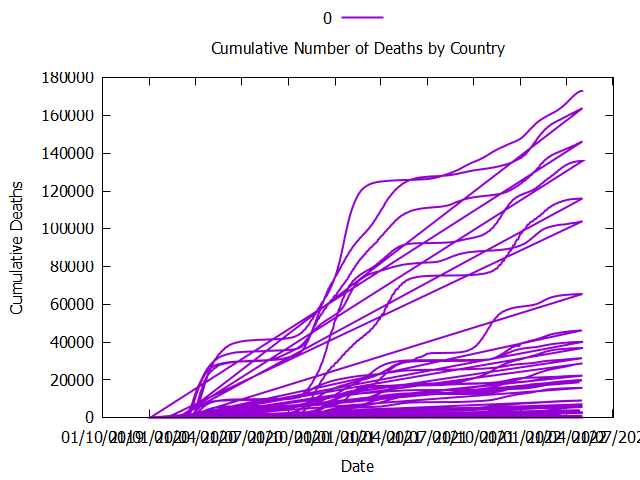
\includegraphics[width=\textwidth]{graph.png}
This script is not perfect, it's a very rough draft to try and get SQL queries and making graphs from them.\\
\\The SQL query is stored in a 'query' variable, it retrieves data from the 'CovidStats' and 'DateInfo' tables. A temporary file is generated with mktemp as part of the requirement, this is stored in a "temp\_data\_file" variable.
The sqlite3 command is executed and it passes the SQL query and the path to the coronavirus.db database file, it returns into 'temp\_data\_file'. The gnuplot script is stored in the "gnuplot\_script" variable. The 'temp\_gnuplot\_script' is used as a temporary file path for the gnuplot script. The gnuplot script creates a graph.png file which is what you're seeing above.
\end{document}
